\documentclass[tikz,border=4pt]{standalone}
\usepackage{libertine}
\usepackage{newtxmath}
\usetikzlibrary{arrows.meta,fit,positioning}

\begin{document}
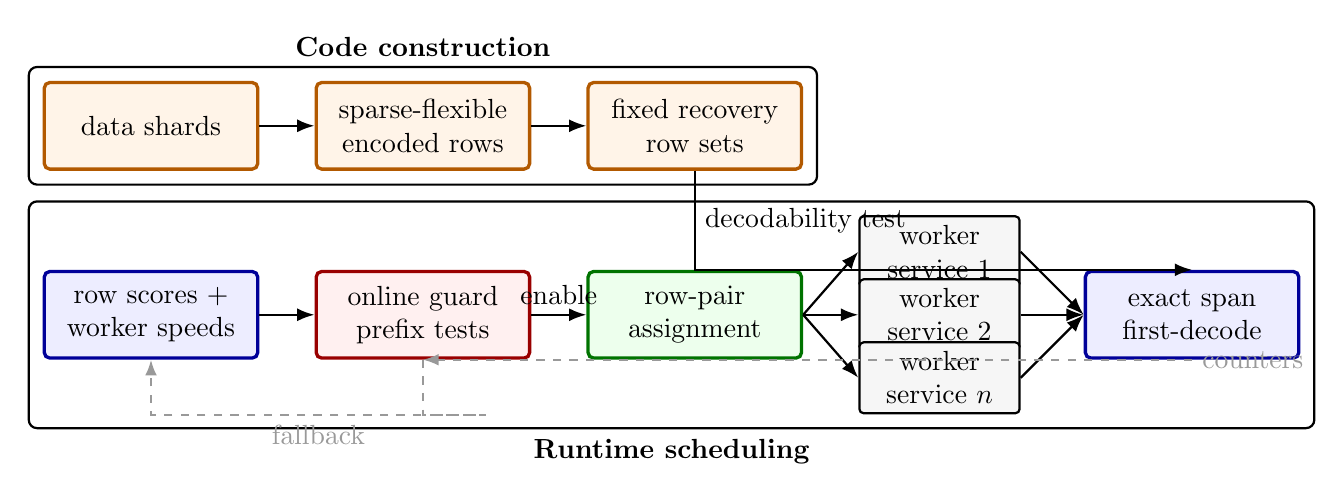
\begin{tikzpicture}[
  font=\normalsize,
  x=1mm,
  y=1mm,
  stage/.style={draw, rounded corners=2pt, very thick, align=center,
    minimum height=11mm, inner sep=3pt},
  code/.style={stage, fill=orange!9, draw=orange!70!black, text width=25mm},
  signal/.style={stage, fill=blue!7, draw=blue!60!black, text width=25mm},
  action/.style={stage, fill=green!7, draw=green!45!black, text width=25mm},
  guardbox/.style={stage, fill=red!6, draw=red!60!black, text width=25mm},
  worker/.style={draw, rounded corners=1.5pt, thick, fill=gray!7,
    align=center, minimum height=7mm, text width=18mm},
  lane/.style={draw, rounded corners=3pt, thick, inner sep=5pt},
  arrow/.style={-{Latex[length=2.2mm]}, thick},
  weakarrow/.style={-{Latex[length=2.0mm]}, thick, dashed, gray!80}
]
  \node[code] (shards) at (0,18) {data shards};
  \node[code, right=7mm of shards] (rows) {sparse-flexible\\encoded rows};
  \node[code, right=7mm of rows] (sets) {fixed recovery\\row sets};
  \node[lane, fit=(shards)(sets), label={[font=\bfseries]above:Code construction}] (codelane) {};

  \node[signal] (features) at (0,-6) {row scores +\\worker speeds};
  \node[guardbox, right=7mm of features] (guard) {online guard\\prefix tests};
  \node[action, right=7mm of guard] (assign) {row-pair\\assignment};
  \node[worker, right=7mm of assign, yshift=8mm] (w1) {worker\\service 1};
  \node[worker, right=7mm of assign] (w2) {worker\\service 2};
  \node[worker, right=7mm of assign, yshift=-8mm] (w3) {worker\\service $n$};
  \node[signal, right=8mm of w2] (monitor) {exact span\\first-decode};
  \node[lane, fit=(features)(guard)(assign)(w1)(w3)(monitor),
    label={[font=\bfseries]below:Runtime scheduling}] (runtimelane) {};

  \draw[arrow] (shards) -- (rows);
  \draw[arrow] (rows) -- (sets);
  \draw[arrow] (features) -- (guard);
  \draw[arrow] (guard) -- node[above] {enable} (assign);
  \draw[weakarrow] (guard.south) |- ++(8,-7) -| node[pos=0.25, below] {fallback}
    (features.south);
  \draw[arrow] (assign.east) -- (w1.west);
  \draw[arrow] (assign.east) -- (w2.west);
  \draw[arrow] (assign.east) -- (w3.west);
  \draw[arrow] (w1.east) -- (monitor.west);
  \draw[arrow] (w2.east) -- (monitor.west);
  \draw[arrow] (w3.east) -- (monitor.west);
  \draw[arrow] (sets.south) |- node[pos=0.25, right] {decodability test}
    (monitor.north);
  \draw[weakarrow] (monitor.south) |- node[pos=0.25, right] {counters}
    (guard.south);
\end{tikzpicture}
\end{document}
